\documentclass[aspectratio=169,11pt]{beamer}
\usetheme{Boadilla}
\usecolortheme{seahorse}
\usepackage{fontspec}
\usepackage{graphicx}
\usepackage{booktabs}
\usepackage{amsmath,amssymb}
\setbeamertemplate{navigation symbols}{}
\setbeamertemplate{caption}{\raggedright\insertcaption\par}
\newcommand{\code}[1]{\texttt{\small\detokenize{#1}}}

\title[Keep/Cull RL]{Süt Sığırcılığında İnek Bazında Keep/Cull Kararı için Pekiştirmeli Öğrenme}
\subtitle{Empirik Stokastik MDP $\cdot$ Q-Learning + DQN}
\author{255172008 --- Artun KARA}
\date{}

\begin{document}

\frame{\titlepage}

\begin{frame}{Problem ve Neden RL?}
\textbf{Problem:} Her ay her inek için \textbf{keep} (elde tut) / \textbf{cull} (sürüden çıkar) kararı; amaç iskontolu uzun vadeli iktisadi getiriyi maksimize etmek.
\vspace{4pt}
\begin{itemize}
\item \textbf{Ardışıklık:} \code{keep} ineği bir sonraki aylık duruma taşır; karar geleceği etkiler.
\item \textbf{Gecikmeli ödül:} Tutmanın değeri gelecekteki süt $-$ birikmiş risk ($\gamma=0.97$).
\item \textbf{Stokastik + büyük uzay:} Geçiş dinamiği gerçek kayıtlardan empirik; 162 durum.
\item \textbf{Neden A*/DP değil:} Ortam stokastik (kod satırıyla ispatlı) $\Rightarrow$ en kısa yol uygulanamaz.
\end{itemize}
\end{frame}

\begin{frame}{MDP Formülasyonu}
\textbf{Durum:} \code{laktasyon_evresi|parite|dim_band|milk_level|milk_trend|health_risk|risk_band} (162 kova).\\
\textbf{Aksiyon:} \code{keep} (0, terminal değil), \code{cull} (1, terminal).
\vspace{4pt}

\textbf{Ödül (kod $\leftrightarrow$ LaTeX birebir):}
\[ R_{\text{keep}} = m\,d\,p - c_b\,d - C_{\text{sağlık}} - C_{\text{üreme}} - C_{\text{beklenen-cull}} \quad(\code{rl_mdp_utils.py:120})\]
\[ R_{\text{cull}} = v_c - c_r - c_{\text{disposal}} \quad(\code{rl_mdp_utils.py:76}) \]
\footnotesize Parametreler \code{reward_baseline_us_2025.csv} (süt fiyatı \& bakım USDA 2025; diğerleri prototip).
\end{frame}

\begin{frame}{Ortam Stokastik (kanıt)}
\code{keep} sonrası bir sonraki durum empirik dağılımdan örneklenir:
\begin{block}{\code{kod/env/rl_experiment_utils.py:161}}
\code{selected = outcomes[int(rng.choice(len(outcomes), p=probabilities))]}
\end{block}
\begin{itemize}
\item \textbf{162 durumun 120'sinde (\%74)} \code{keep} altında birden çok olası $s'$ var.
\item Örn: bir durum 3 farklı $s'$'ye her biri $p=0.333$ ile geçer.
\item \code{cull} deterministik terminal. Aynı seed $\to$ aynı yörünge (sadece tekrarlanabilirlik).
\end{itemize}
\end{frame}

\begin{frame}{Yöntem ve Deney Kurulumu}
\begin{columns}
\begin{column}{0.52\textwidth}
\textbf{Ajanlar / referans:}
\begin{itemize}\small
\item Tabular Q-Learning (\textbf{off-policy})
\item SB3 DQN (off-policy, replay buffer)
\item MDP Value Iteration (optimum ref.)
\item Baseline: random / keep\_all / cull\_all / risk\_threshold
\end{itemize}
\end{column}
\begin{column}{0.48\textwidth}
\textbf{Kurulum:}
\begin{itemize}\small
\item Seedler: 42,123,2024,7,99 ($\geq 5$)
\item \code{full}: DQN 100k, Q 4000 ep.
\item \code{np.random.default_rng} (yasak yok)
\item Eval: deterministic/greedy, 500 ep/seed
\end{itemize}
\end{column}
\end{columns}
\end{frame}

\begin{frame}{Sonuçlar (seed ort. $\pm$ std, full)}
\centering
\begin{tabular}{@{}llrrr@{}}
\toprule
Politika & Tür & Getiri (USD) & Std & Cull \\
\midrule
\textbf{qlearning} & ajan & \textbf{-204} & 30 & 0.72 \\
mdp\_value\_iteration & referans & -225 & 42 & 0.45 \\
\textbf{dqn} & ajan & \textbf{-270} & 20 & 0.82 \\
risk\_threshold & baseline & -385 & 53 & 0.85 \\
keep\_all & baseline & -428 & 34 & 0.00 \\
random\_policy & baseline & -964 & 56 & 0.75 \\
cull\_all & baseline & -1300 & 0 & 1.00 \\
\bottomrule
\end{tabular}
\vspace{4pt}
\footnotesize Ajanlar tüm baselineları geçti; \textbf{Q-learning model-tabanlı optimuma istatistiksel olarak eşitlendi} (fark anlamsız, eşli $t$-test $p\approx0.37$). Dağılım sağa çarpık: medyan $-556$ vs ort. $-204$.
\end{frame}

\begin{frame}{Grafik 1 --- Öğrenme Eğrisi}
\centering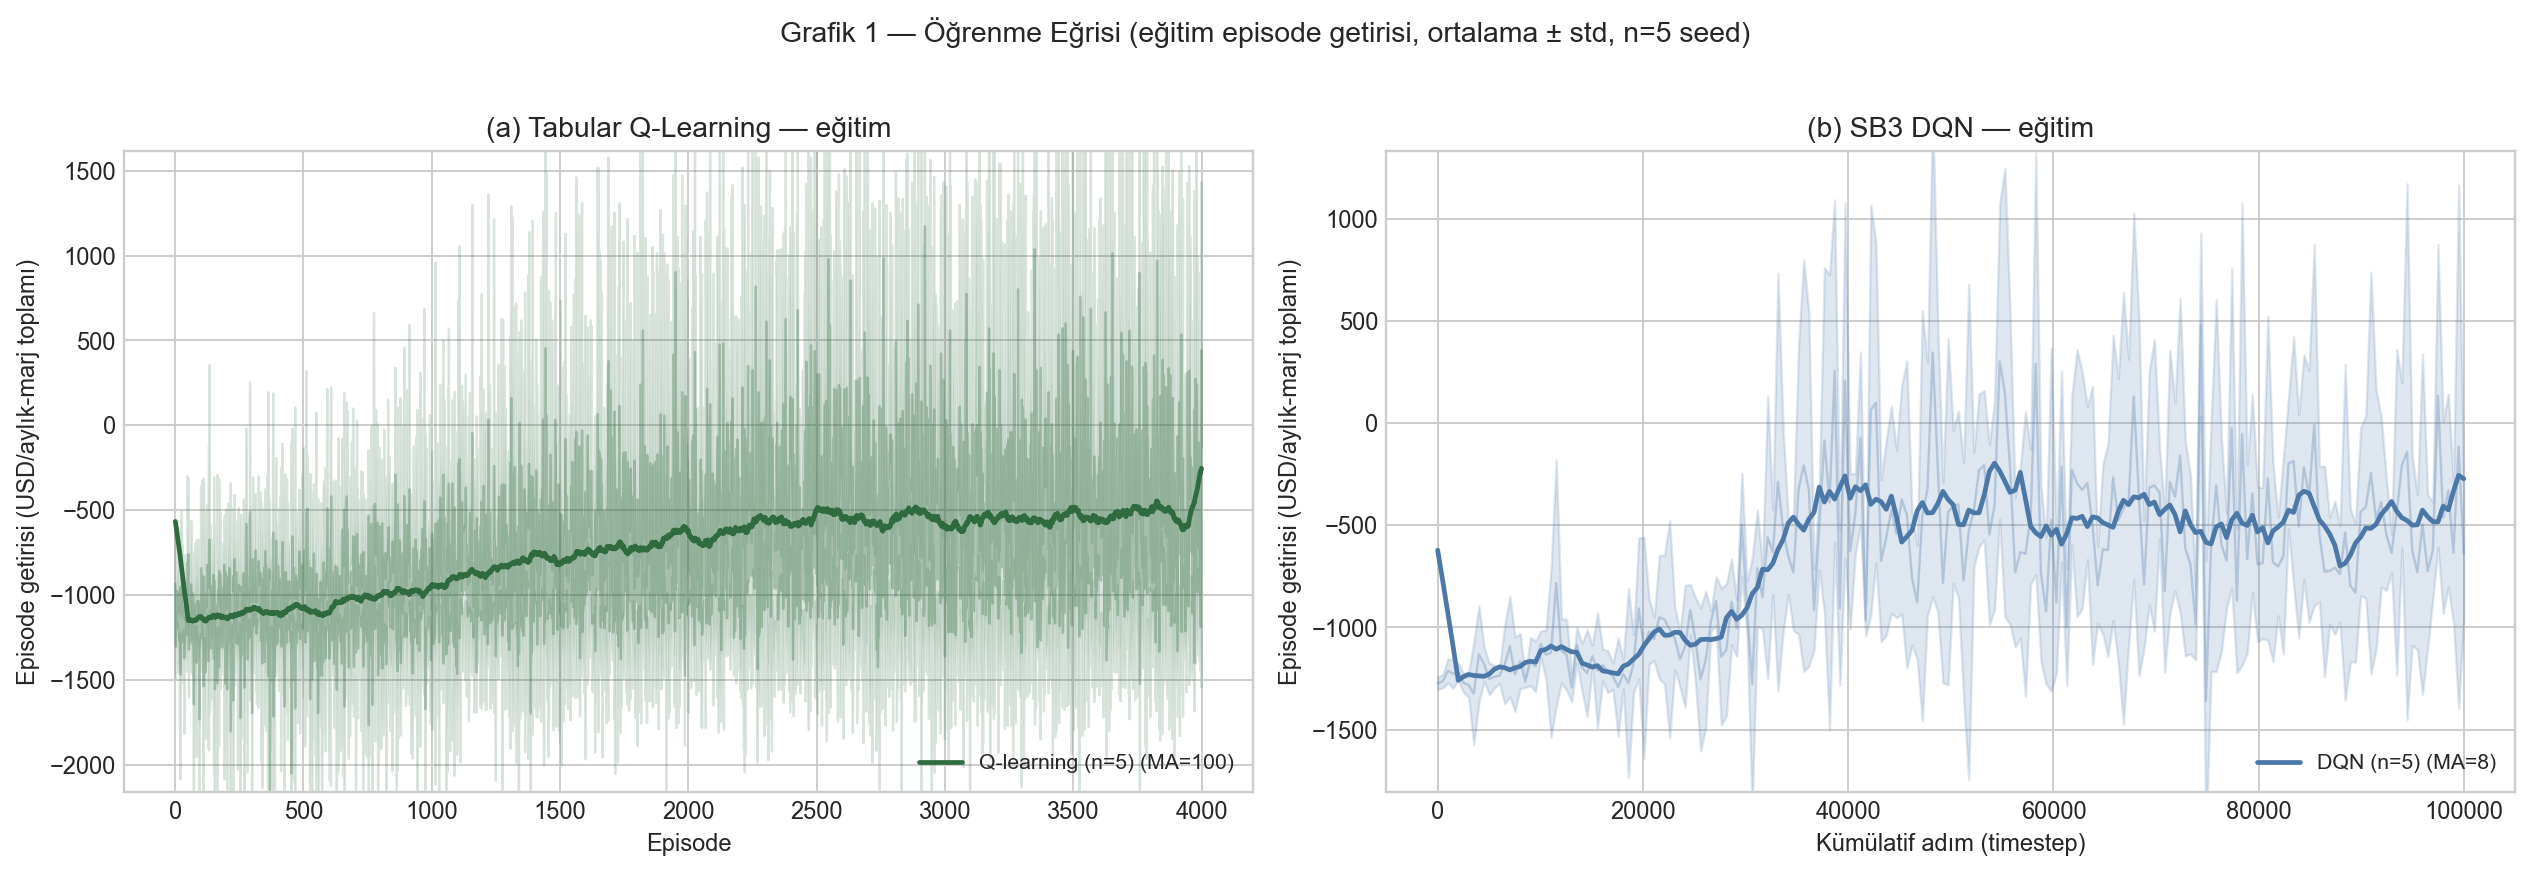
\includegraphics[width=0.92\textwidth]{grafikler/01_ogrenme_egrisi.png}\\
\footnotesize y: episode getirisi (anlık ödül değil); n=5 seed, ort.$\pm$std + hareketli ortalama.
\end{frame}

\begin{frame}{Grafik 2 --- Test/Eval Eğrisi}
\centering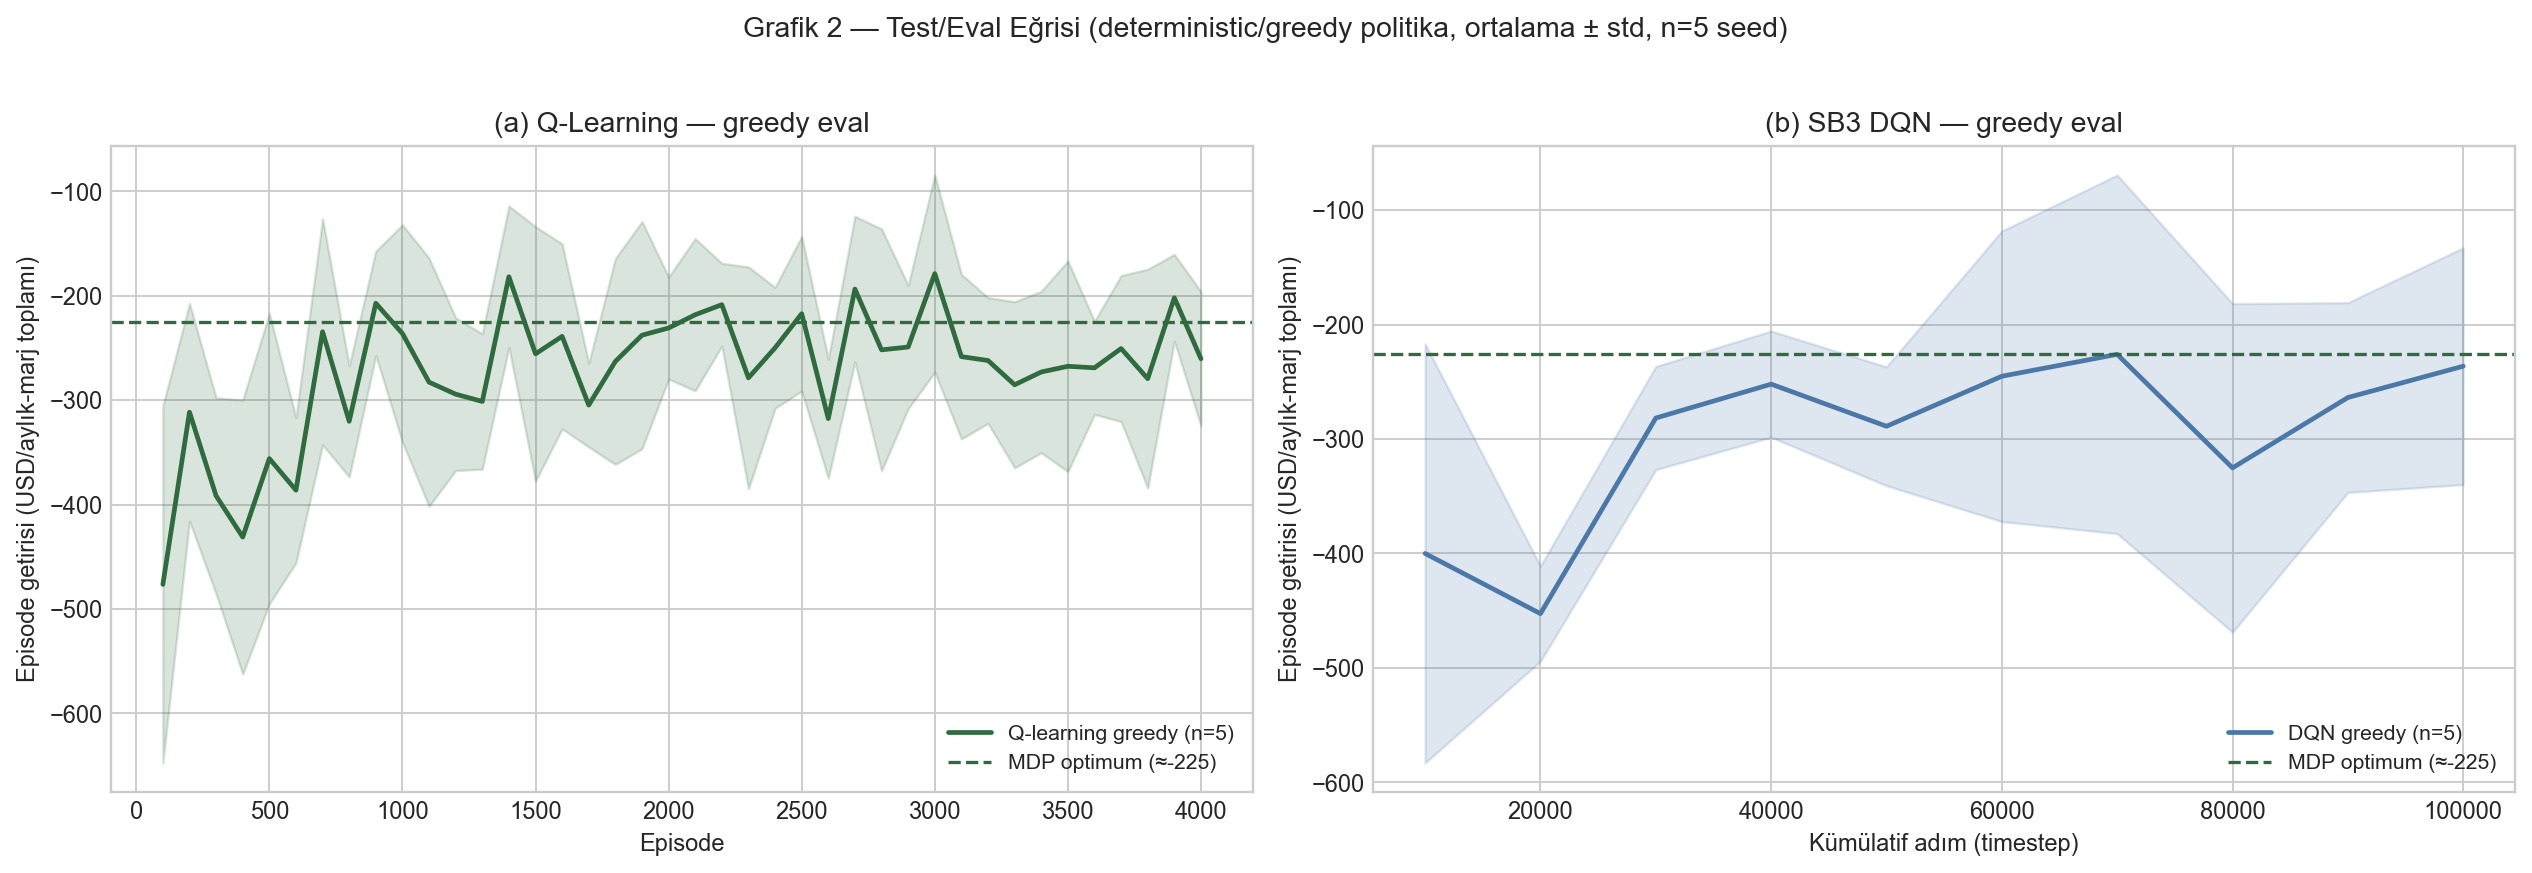
\includegraphics[width=0.92\textwidth]{grafikler/02_eval_egrisi.png}\\
\footnotesize Deterministic/greedy; yeşil kesik çizgi MDP-optimum referansı (tavan). Ajanlar tavana ulaşıyor.
\end{frame}

\begin{frame}{Grafik 3 --- Loss + Policy Heatmap}
\centering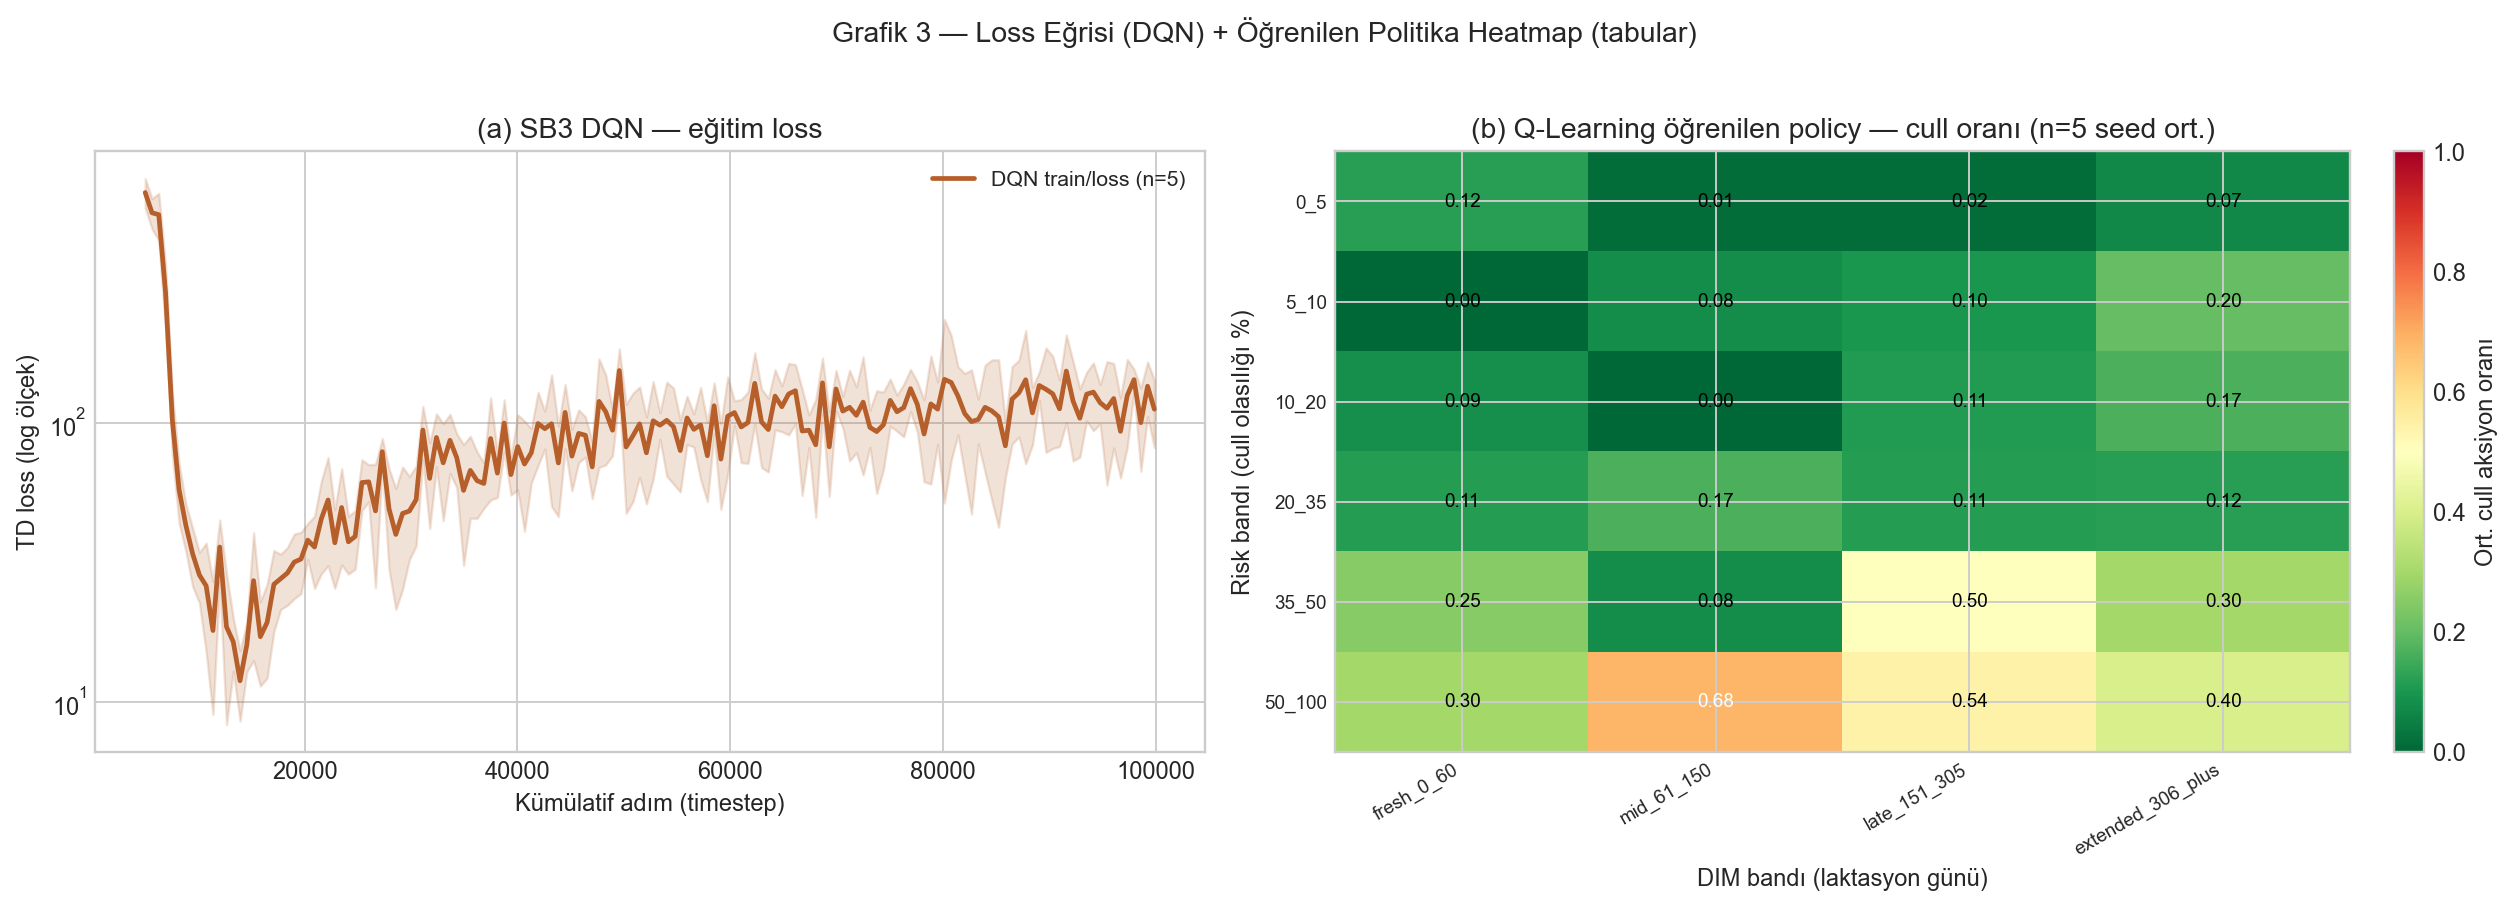
\includegraphics[width=0.92\textwidth]{grafikler/03_loss_ve_policy_heatmap.png}\\
\footnotesize DQN TD-loss yakınsıyor; heatmap: yüksek risk $\times$ ileri DIM $\to$ cull oranı artıyor (iktisadi olarak anlamlı).
\end{frame}

\begin{frame}{Grafik 4 --- Hiperparametre Duyarlılığı}
\centering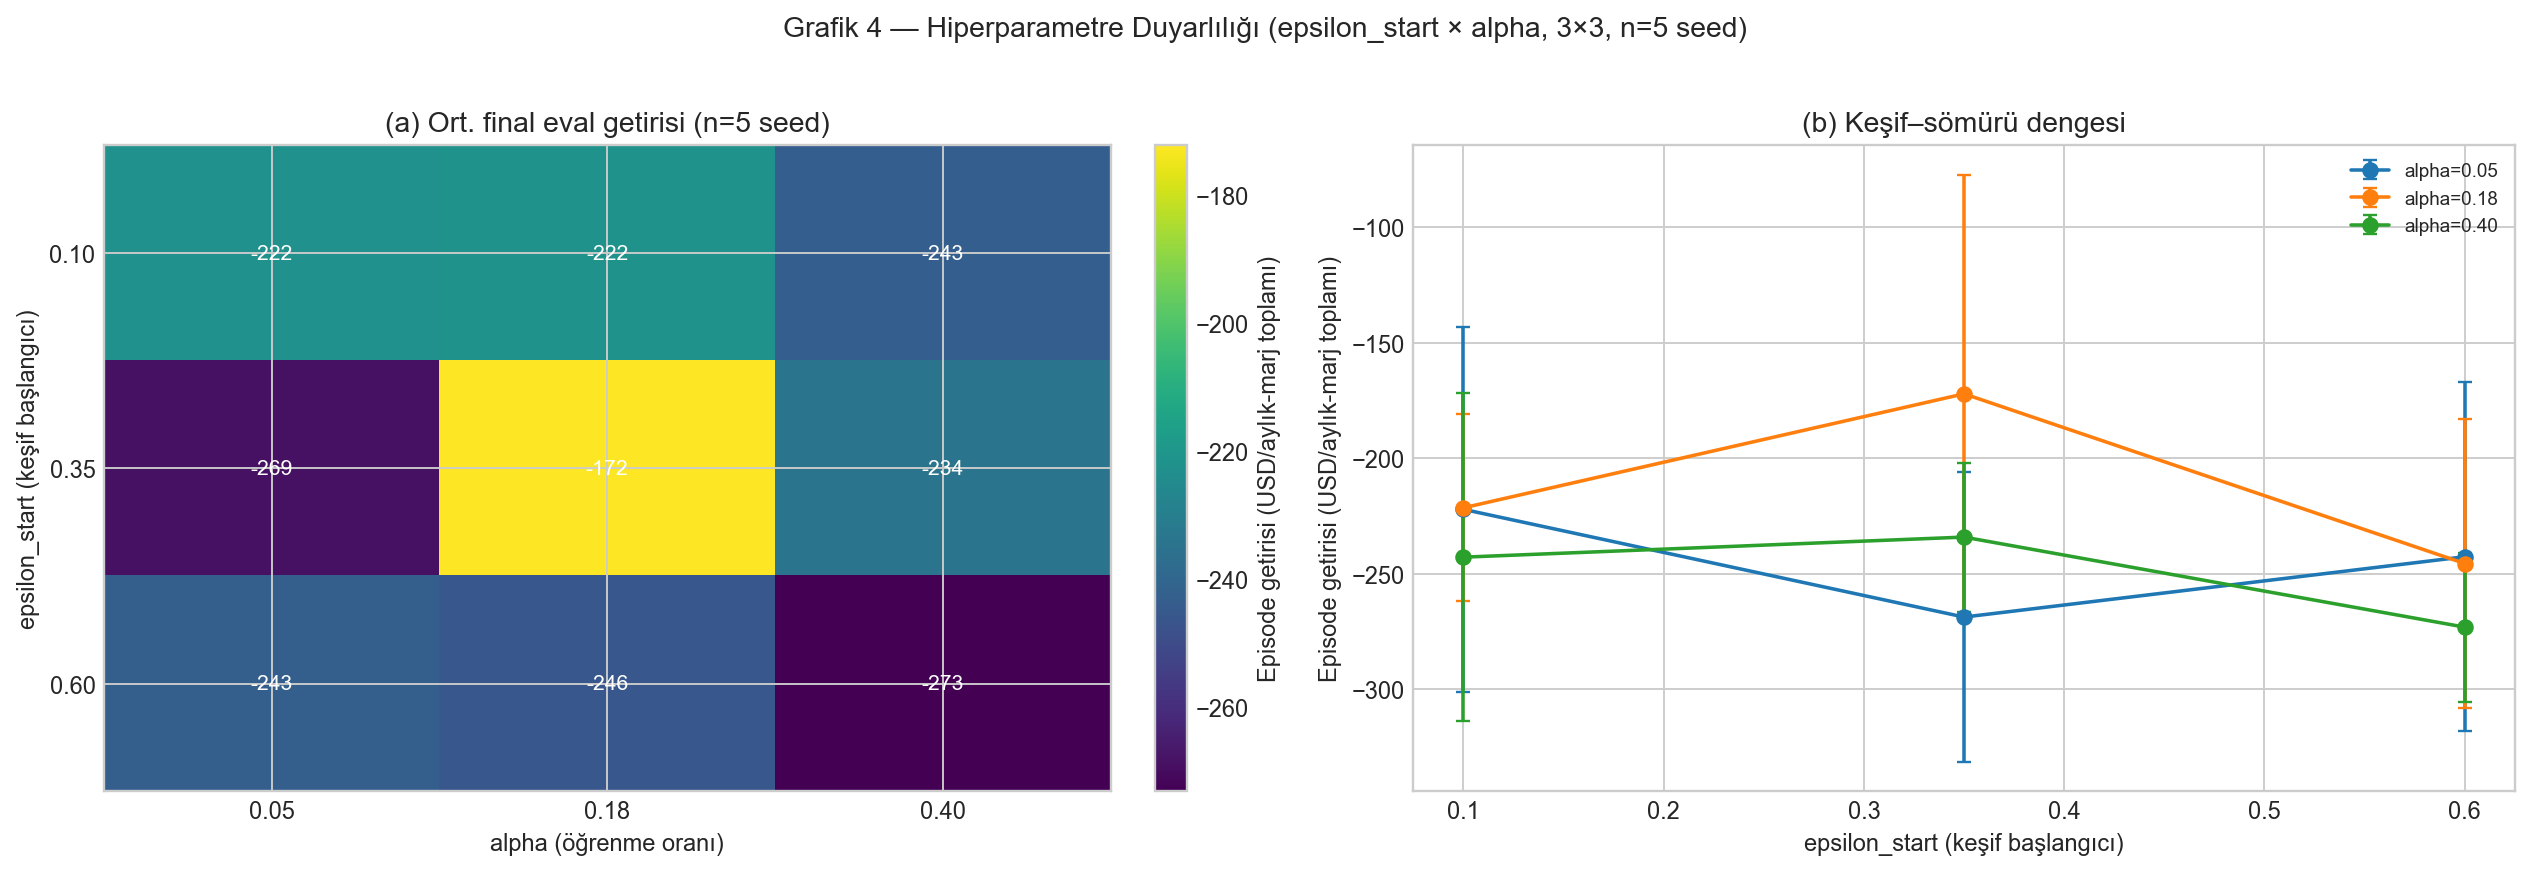
\includegraphics[width=0.92\textwidth]{grafikler/04_hiperparametre_duyarlilik.png}\\
\footnotesize Sweet-spot: orta keşif $\times$ orta öğrenme oranı ($\varepsilon_0=0.35,\ \alpha=0.18$) = seçilen varsayılanlar.
\end{frame}

\begin{frame}{Grafik 5 --- Baseline Karşılaştırma}
\centering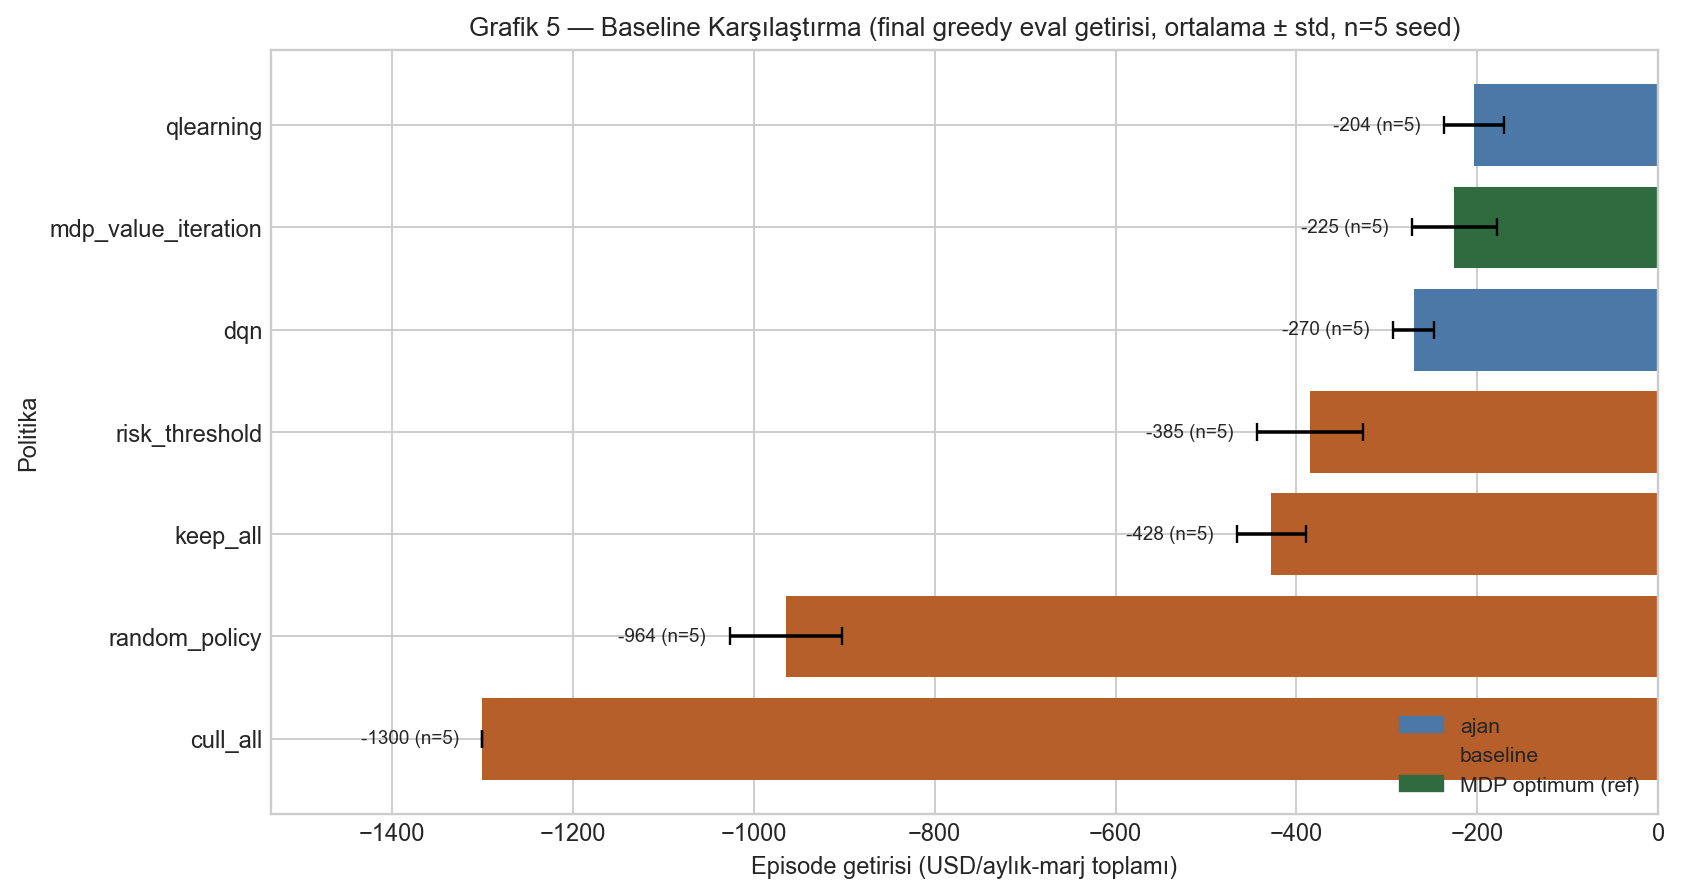
\includegraphics[width=0.74\textwidth]{grafikler/05_baseline_karsilastirma.png}\\
\footnotesize Eğitilmiş ajanlar (mavi) tüm naif/heuristik baselineları (turuncu) geçiyor; MDP optimum yeşil referans.
\end{frame}

\begin{frame}{Teslim-3 Savunma --- Özet (kod satırlı)}
\begin{itemize}\small
\item \textbf{Stokastik}: \code{keep} için empirik $p(s'|s,a)$ (\code{rl_experiment_utils.py:161}); \%74 durumda $>1$ olası $s'$.
\item \textbf{Off-policy}: Q-learning davranış $\varepsilon$-greedy (\code{rl_core.py:309}) vs hedef $\max_a Q$ (\code{:321}); DQN replay buffer (\code{:474}). Online $\neq$ offline.
\item \textbf{Markov}: \code{state_bucket}$\to$\code{next} varsayımı; trend/risk geçmişi özetler $\to$ \emph{yaklaşık} Markov (bucketing kaybı).
\item \textbf{POMDP}: \code{cull_risk} = denetimli tahmin (gerçek değil); feature engineering ile gözlemi Markov'a yaklaştırma.
\end{itemize}
\end{frame}

\begin{frame}{Sonuç}
\begin{itemize}
\item Empirik, stokastik, gecikmeli-ödüllü keep/cull ortamı $\Rightarrow$ RL gerekçeli.
\item Q-Learning ve DQN, $\geq 5$ seed üzerinde tüm baselineları geçti; model-tabanlı optimuma istatistiksel olarak eşitlendi (fark anlamsız).
\item Tüm sonuçlar tek komutla (\code{run_all.sh}) yeniden üretilebilir; ham loglardan doğrulanabilir.
\end{itemize}
\vspace{8pt}
\centering\Large Teşekkürler.
\end{frame}

\end{document}
